---
id: tkz-euclide-ejemplo-02
title: Recta Numérica
description: "Dibuja una recta numérica sobre el eje x con marcas y etiquetas."
keywords: [recta, numerica, eje, coordenadas]
tags: [tkzInit,tkzDrawX,tkzLabelX]
sort: 2
---
\documentclass[tikz,border=2mm]{standalone}
\usepackage{tkz-base}
\usepackage{tkz-euclide}

\begin{document}
    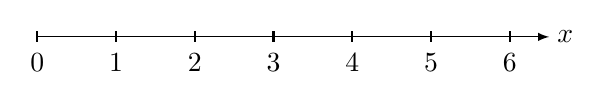
\begin{tikzpicture}
        % Define el sistema de coordenadas ortogonales.
        \tkzInit[xmin=0,xmax=6]
        
        % Dibuja el eje x, etiqueta a la derecha
        \tkzDrawX[right=2pt]
        
        % Coloca etiquetas/graduaciones en el eje x
        \tkzLabelX
    \end{tikzpicture}
\end{document}